\documentclass[twoside]{book}

% Packages required by doxygen
\usepackage{calc}
\usepackage{doxygen}
\usepackage{graphicx}
\usepackage[utf8]{inputenc}
\usepackage{makeidx}
\usepackage{multicol}
\usepackage{multirow}
\usepackage{textcomp}
\usepackage[table]{xcolor}

% Font selection
\usepackage[T1]{fontenc}
\usepackage{mathptmx}
\usepackage[scaled=.90]{helvet}
\usepackage{courier}
\usepackage{amssymb}
\usepackage{sectsty}
\renewcommand{\familydefault}{\sfdefault}
\allsectionsfont{%
  \fontseries{bc}\selectfont%
  \color{darkgray}%
}
\renewcommand{\DoxyLabelFont}{%
  \fontseries{bc}\selectfont%
  \color{darkgray}%
}

% Page & text layout
\usepackage{geometry}
\geometry{%
  a4paper,%
  top=2.5cm,%
  bottom=2.5cm,%
  left=2.5cm,%
  right=2.5cm%
}
\tolerance=750
\hfuzz=15pt
\hbadness=750
\setlength{\emergencystretch}{15pt}
\setlength{\parindent}{0cm}
\setlength{\parskip}{0.2cm}
\makeatletter
\renewcommand{\paragraph}{%
  \@startsection{paragraph}{4}{0ex}{-1.0ex}{1.0ex}{%
    \normalfont\normalsize\bfseries\SS@parafont%
  }%
}
\renewcommand{\subparagraph}{%
  \@startsection{subparagraph}{5}{0ex}{-1.0ex}{1.0ex}{%
    \normalfont\normalsize\bfseries\SS@subparafont%
  }%
}
\makeatother

% Headers & footers
\usepackage{fancyhdr}
\pagestyle{fancyplain}
\fancyhead[LE]{\fancyplain{}{\bfseries\thepage}}
\fancyhead[CE]{\fancyplain{}{}}
\fancyhead[RE]{\fancyplain{}{\bfseries\leftmark}}
\fancyhead[LO]{\fancyplain{}{\bfseries\rightmark}}
\fancyhead[CO]{\fancyplain{}{}}
\fancyhead[RO]{\fancyplain{}{\bfseries\thepage}}
\fancyfoot[LE]{\fancyplain{}{}}
\fancyfoot[CE]{\fancyplain{}{}}
\fancyfoot[RE]{\fancyplain{}{\bfseries\scriptsize Generated on Mon Jun 22 2015 20\-:59\-:21 for My Project by Doxygen }}
\fancyfoot[LO]{\fancyplain{}{\bfseries\scriptsize Generated on Mon Jun 22 2015 20\-:59\-:21 for My Project by Doxygen }}
\fancyfoot[CO]{\fancyplain{}{}}
\fancyfoot[RO]{\fancyplain{}{}}
\renewcommand{\footrulewidth}{0.4pt}
\renewcommand{\chaptermark}[1]{%
  \markboth{#1}{}%
}
\renewcommand{\sectionmark}[1]{%
  \markright{\thesection\ #1}%
}

% Indices & bibliography
\usepackage{natbib}
\usepackage[titles]{tocloft}
\setcounter{tocdepth}{3}
\setcounter{secnumdepth}{5}
\makeindex

% Hyperlinks (required, but should be loaded last)
\usepackage{ifpdf}
\ifpdf
  \usepackage[pdftex,pagebackref=true]{hyperref}
\else
  \usepackage[ps2pdf,pagebackref=true]{hyperref}
\fi
\hypersetup{%
  colorlinks=true,%
  linkcolor=blue,%
  citecolor=blue,%
  unicode%
}

% Custom commands
\newcommand{\clearemptydoublepage}{%
  \newpage{\pagestyle{empty}\cleardoublepage}%
}


%===== C O N T E N T S =====

\begin{document}

% Titlepage & ToC
\hypersetup{pageanchor=false}
\pagenumbering{roman}
\begin{titlepage}
\vspace*{7cm}
\begin{center}%
{\Large My Project }\\
\vspace*{1cm}
{\large Generated by Doxygen 1.8.6}\\
\vspace*{0.5cm}
{\small Mon Jun 22 2015 20:59:21}\\
\end{center}
\end{titlepage}
\clearemptydoublepage
\tableofcontents
\clearemptydoublepage
\pagenumbering{arabic}
\hypersetup{pageanchor=true}

%--- Begin generated contents ---
\chapter{Hierarchical Index}
\section{Class Hierarchy}
This inheritance list is sorted roughly, but not completely, alphabetically\-:\begin{DoxyCompactList}
\item \contentsline{section}{C\-Brick}{\pageref{classCBrick}}{}
\begin{DoxyCompactList}
\item \contentsline{section}{C\-I\-Brick}{\pageref{classCIBrick}}{}
\item \contentsline{section}{C\-L\-Brick}{\pageref{classCLBrick}}{}
\item \contentsline{section}{C\-O\-Brick}{\pageref{classCOBrick}}{}
\item \contentsline{section}{C\-S\-Brick}{\pageref{classCSBrick}}{}
\item \contentsline{section}{C\-T\-Brick}{\pageref{classCTBrick}}{}
\end{DoxyCompactList}
\item \contentsline{section}{C\-Brick\-Factory}{\pageref{classCBrickFactory}}{}
\item \contentsline{section}{C\-Event\-Handler}{\pageref{classCEventHandler}}{}
\item \contentsline{section}{C\-Game}{\pageref{classCGame}}{}
\item \contentsline{section}{C\-Main\-Grid}{\pageref{classCMainGrid}}{}
\item \contentsline{section}{C\-Orientation}{\pageref{classCOrientation}}{}
\item \contentsline{section}{C\-Picture}{\pageref{classCPicture}}{}
\item \contentsline{section}{C\-Point}{\pageref{classCPoint}}{}
\begin{DoxyCompactList}
\item \contentsline{section}{C\-Button}{\pageref{classCButton}}{}
\item \contentsline{section}{C\-Rectangle}{\pageref{classCRectangle}}{}
\end{DoxyCompactList}
\item \contentsline{section}{C\-Position}{\pageref{classCPosition}}{}
\item \contentsline{section}{C\-S\-D\-L\-Wrapper}{\pageref{classCSDLWrapper}}{}
\item \contentsline{section}{C\-Slab}{\pageref{classCSlab}}{}
\item \contentsline{section}{C\-Table\-Coor}{\pageref{classCTableCoor}}{}
\item \contentsline{section}{C\-Time\-Mod}{\pageref{classCTimeMod}}{}
\end{DoxyCompactList}

\chapter{Class Index}
\section{Class List}
Here are the classes, structs, unions and interfaces with brief descriptions\-:\begin{DoxyCompactList}
\item\contentsline{section}{\hyperlink{classCBrick}{C\-Brick} }{\pageref{classCBrick}}{}
\item\contentsline{section}{\hyperlink{classCBrickFactory}{C\-Brick\-Factory} }{\pageref{classCBrickFactory}}{}
\item\contentsline{section}{\hyperlink{classCButton}{C\-Button} }{\pageref{classCButton}}{}
\item\contentsline{section}{\hyperlink{classCEventHandler}{C\-Event\-Handler} }{\pageref{classCEventHandler}}{}
\item\contentsline{section}{\hyperlink{classCGame}{C\-Game} }{\pageref{classCGame}}{}
\item\contentsline{section}{\hyperlink{classCIBrick}{C\-I\-Brick} }{\pageref{classCIBrick}}{}
\item\contentsline{section}{\hyperlink{classCLBrick}{C\-L\-Brick} }{\pageref{classCLBrick}}{}
\item\contentsline{section}{\hyperlink{classCMainGrid}{C\-Main\-Grid} }{\pageref{classCMainGrid}}{}
\item\contentsline{section}{\hyperlink{classCOBrick}{C\-O\-Brick} }{\pageref{classCOBrick}}{}
\item\contentsline{section}{\hyperlink{classCOrientation}{C\-Orientation} }{\pageref{classCOrientation}}{}
\item\contentsline{section}{\hyperlink{classCPicture}{C\-Picture} }{\pageref{classCPicture}}{}
\item\contentsline{section}{\hyperlink{classCPoint}{C\-Point} }{\pageref{classCPoint}}{}
\item\contentsline{section}{\hyperlink{classCPosition}{C\-Position} }{\pageref{classCPosition}}{}
\item\contentsline{section}{\hyperlink{classCRectangle}{C\-Rectangle} }{\pageref{classCRectangle}}{}
\item\contentsline{section}{\hyperlink{classCSBrick}{C\-S\-Brick} }{\pageref{classCSBrick}}{}
\item\contentsline{section}{\hyperlink{classCSDLWrapper}{C\-S\-D\-L\-Wrapper} }{\pageref{classCSDLWrapper}}{}
\item\contentsline{section}{\hyperlink{classCSlab}{C\-Slab} }{\pageref{classCSlab}}{}
\item\contentsline{section}{\hyperlink{classCTableCoor}{C\-Table\-Coor} }{\pageref{classCTableCoor}}{}
\item\contentsline{section}{\hyperlink{classCTBrick}{C\-T\-Brick} }{\pageref{classCTBrick}}{}
\item\contentsline{section}{\hyperlink{classCTimeMod}{C\-Time\-Mod} }{\pageref{classCTimeMod}}{}
\end{DoxyCompactList}

\chapter{Class Documentation}
\hypertarget{classCBrick}{\section{C\-Brick Class Reference}
\label{classCBrick}\index{C\-Brick@{C\-Brick}}
}
Inheritance diagram for C\-Brick\-:\begin{figure}[H]
\begin{center}
\leavevmode
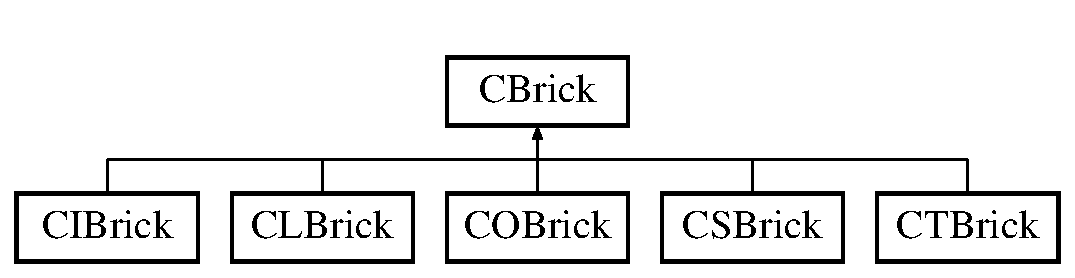
\includegraphics[height=2.000000cm]{classCBrick}
\end{center}
\end{figure}
\subsection*{Public Member Functions}
\begin{DoxyCompactItemize}
\item 
\hypertarget{classCBrick_a7e9a7be334cf5fd214135c73188e5e3c}{{\bfseries C\-Brick} (Brick\-Types typeof\-Brick, const Direction direction=Direction\-::\-R)}\label{classCBrick_a7e9a7be334cf5fd214135c73188e5e3c}

\item 
\hypertarget{classCBrick_a384bfcee237653f7ee52424ae892036c}{{\bfseries C\-Brick} (const std\-::vector$<$ \hyperlink{classCSlab}{C\-Slab} $>$ \&blocks, const Direction direction=Direction\-::\-R)}\label{classCBrick_a384bfcee237653f7ee52424ae892036c}

\item 
\hypertarget{classCBrick_a6036490c7d05a6d7cf0a82aa492019d5}{{\bfseries C\-Brick} (const \hyperlink{classCBrick}{C\-Brick} \&brick)}\label{classCBrick_a6036490c7d05a6d7cf0a82aa492019d5}

\item 
\hypertarget{classCBrick_a8d2b23220a7ce8a9edc6f1570105ed4f}{Coordinatest\-List {\bfseries Get\-Block\-Positions} () const }\label{classCBrick_a8d2b23220a7ce8a9edc6f1570105ed4f}

\item 
\hypertarget{classCBrick_a52d81e87ea62278fb2f06fcbf76217ea}{void {\bfseries Move} (const Direction direction=Direction\-::\-D)}\label{classCBrick_a52d81e87ea62278fb2f06fcbf76217ea}

\item 
\hypertarget{classCBrick_ab80db254175cc8f3fb7f9359f9009ef0}{virtual void {\bfseries Rotate} (const bool clock\-Wise=true)=0}\label{classCBrick_ab80db254175cc8f3fb7f9359f9009ef0}

\item 
\hypertarget{classCBrick_a2db8a43893f212040daa6716c51d63fc}{Brick\-Types {\bfseries Get\-Block\-Type} () const }\label{classCBrick_a2db8a43893f212040daa6716c51d63fc}

\end{DoxyCompactItemize}
\subsection*{Static Public Member Functions}
\begin{DoxyCompactItemize}
\item 
\hypertarget{classCBrick_ac96d1acb6be0e541a84bf8d4ab53d3fd}{static void {\bfseries Set\-Background\-Image} (const Path \&path)}\label{classCBrick_ac96d1acb6be0e541a84bf8d4ab53d3fd}

\item 
\hypertarget{classCBrick_ad372d76a714fba18332748825145c675}{static const String {\bfseries Get\-Image} ()}\label{classCBrick_ad372d76a714fba18332748825145c675}

\end{DoxyCompactItemize}
\subsection*{Protected Attributes}
\begin{DoxyCompactItemize}
\item 
\hypertarget{classCBrick_a8204bd386e65da4bbb6dbe1a0f973535}{std\-::vector$<$ \hyperlink{classCSlab}{C\-Slab} $>$ {\bfseries m\-\_\-blocks}}\label{classCBrick_a8204bd386e65da4bbb6dbe1a0f973535}

\item 
\hypertarget{classCBrick_a61a9a82c266c4f0986833426e20fc583}{\hyperlink{classCOrientation}{C\-Orientation} {\bfseries m\-\_\-direction}}\label{classCBrick_a61a9a82c266c4f0986833426e20fc583}

\end{DoxyCompactItemize}


The documentation for this class was generated from the following files\-:\begin{DoxyCompactItemize}
\item 
inc/Brick.\-h\item 
src/Brick.\-cpp\end{DoxyCompactItemize}

\hypertarget{classCBrickFactory}{\section{C\-Brick\-Factory Class Reference}
\label{classCBrickFactory}\index{C\-Brick\-Factory@{C\-Brick\-Factory}}
}
\subsection*{Static Public Member Functions}
\begin{DoxyCompactItemize}
\item 
\hypertarget{classCBrickFactory_aae7645738f3d60ad8ce2cefe03d012f2}{static \hyperlink{classCBrick}{C\-Brick} $\ast$ {\bfseries Get\-Brick} (const Brick\-Types brick\-Type)}\label{classCBrickFactory_aae7645738f3d60ad8ce2cefe03d012f2}

\item 
\hypertarget{classCBrickFactory_ae6f2aa7d151bb01972ac42da029ef5b9}{static \hyperlink{classCBrick}{C\-Brick} $\ast$ {\bfseries Get\-Random\-Brick} ()}\label{classCBrickFactory_ae6f2aa7d151bb01972ac42da029ef5b9}

\end{DoxyCompactItemize}


The documentation for this class was generated from the following files\-:\begin{DoxyCompactItemize}
\item 
inc/Brick\-Factory.\-h\item 
src/Brick\-Factory.\-cpp\end{DoxyCompactItemize}

\hypertarget{classCButton}{\section{C\-Button Class Reference}
\label{classCButton}\index{C\-Button@{C\-Button}}
}
Inheritance diagram for C\-Button\-:\begin{figure}[H]
\begin{center}
\leavevmode
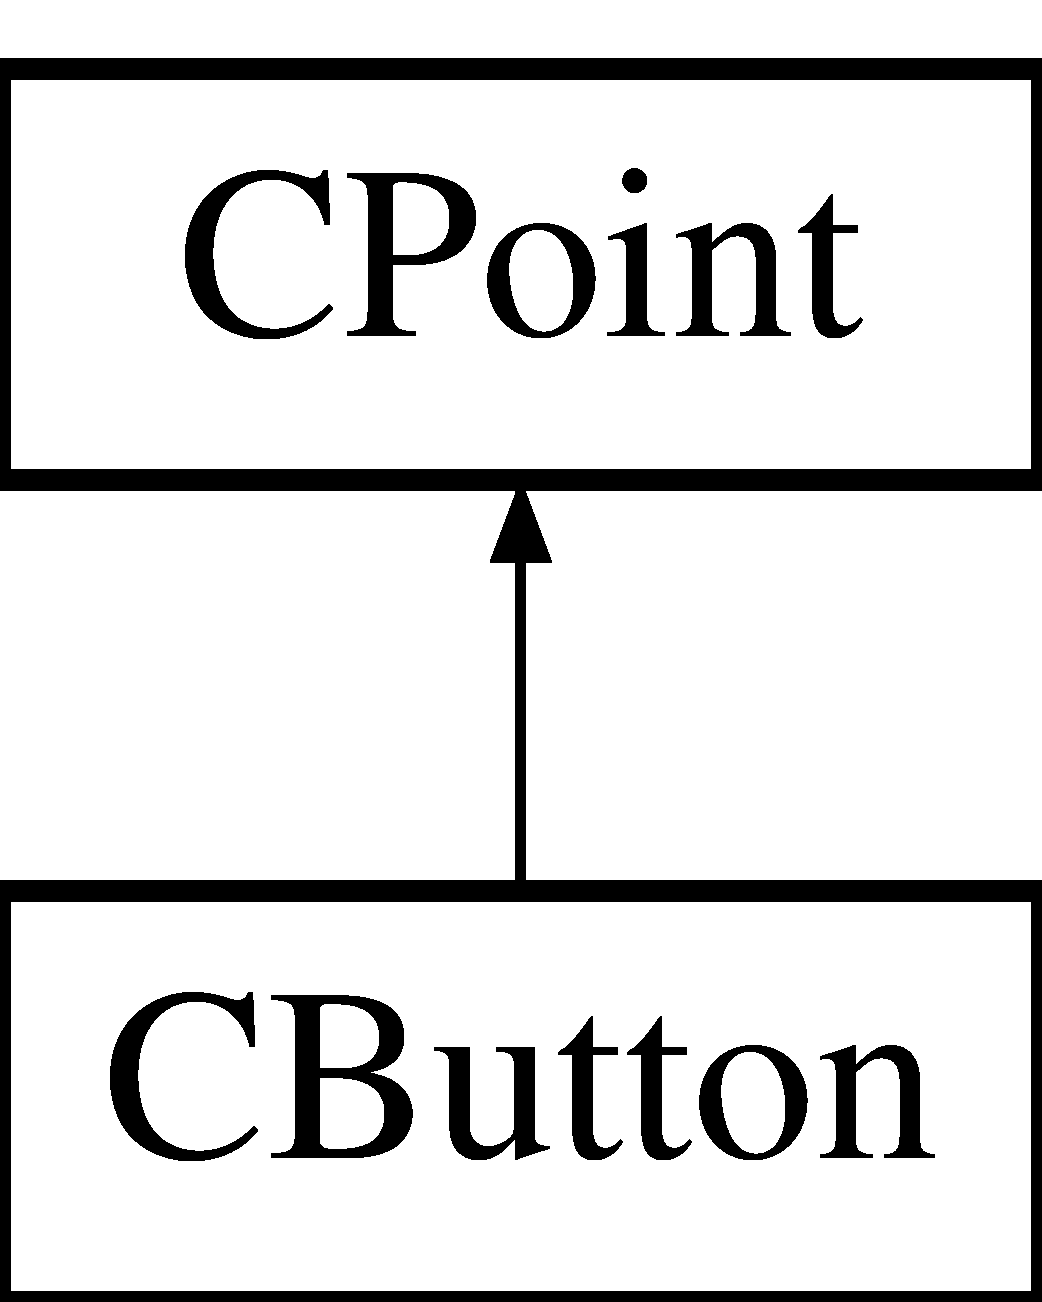
\includegraphics[height=2.000000cm]{classCButton}
\end{center}
\end{figure}
\subsection*{Public Member Functions}
\begin{DoxyCompactItemize}
\item 
\hypertarget{classCButton_a9c8a3e8bd97e29a94897ecb334f8d271}{{\bfseries C\-Button} (C\-U\-Int x, C\-U\-Int y, const String \&button\-Name=\char`\"{}dummy\char`\"{}, const Path \&button\-Location=\char`\"{}\char`\"{})}\label{classCButton_a9c8a3e8bd97e29a94897ecb334f8d271}

\item 
\hypertarget{classCButton_adfb3b62e942861d79cab77bce379de8f}{String {\bfseries Get\-Path} () const }\label{classCButton_adfb3b62e942861d79cab77bce379de8f}

\end{DoxyCompactItemize}


The documentation for this class was generated from the following files\-:\begin{DoxyCompactItemize}
\item 
inc/Button.\-h\item 
src/Button.\-cpp\end{DoxyCompactItemize}

\hypertarget{classCEventHandler}{\section{C\-Event\-Handler Class Reference}
\label{classCEventHandler}\index{C\-Event\-Handler@{C\-Event\-Handler}}
}
\subsection*{Public Member Functions}
\begin{DoxyCompactItemize}
\item 
\hypertarget{classCEventHandler_a4aa21f21c987d79b17ca7dbfebb465f2}{void {\bfseries Add\-Quit\-Action\-Handler} (std\-::function$<$ void()$>$ callback)}\label{classCEventHandler_a4aa21f21c987d79b17ca7dbfebb465f2}

\item 
\hypertarget{classCEventHandler_a3e1d6d4555c196e3a46ae02534f8306f}{void {\bfseries Main\-Event\-Loop} ()}\label{classCEventHandler_a3e1d6d4555c196e3a46ae02534f8306f}

\end{DoxyCompactItemize}


The documentation for this class was generated from the following files\-:\begin{DoxyCompactItemize}
\item 
inc/Event\-Handler.\-h\item 
src/Event\-Handler.\-cpp\end{DoxyCompactItemize}

\hypertarget{classCGame}{\section{C\-Game Class Reference}
\label{classCGame}\index{C\-Game@{C\-Game}}
}
\subsection*{Public Member Functions}
\begin{DoxyCompactItemize}
\item 
\hypertarget{classCGame_a4da7ce24984c52382edb77b7b6271e56}{void {\bfseries Initialize} (C\-U\-Int rows\-Count=50, C\-U\-Int columns\-Count=10)}\label{classCGame_a4da7ce24984c52382edb77b7b6271e56}

\item 
\hypertarget{classCGame_a04641889f2aa31b7742158d9246bf3bd}{void {\bfseries Init\-Window} (C\-U\-Int width=600, C\-U\-Int height=400)}\label{classCGame_a04641889f2aa31b7742158d9246bf3bd}

\item 
\hypertarget{classCGame_a16f0e8ee75a18c3b8e2044069bb8d12d}{void {\bfseries Show\-Grid} ()}\label{classCGame_a16f0e8ee75a18c3b8e2044069bb8d12d}

\item 
\hypertarget{classCGame_a526664bc74d203e16962372fb850328e}{void {\bfseries Main\-Loop} ()}\label{classCGame_a526664bc74d203e16962372fb850328e}

\item 
\hypertarget{classCGame_af11fa563908ad1685e836b5c375242ab}{void {\bfseries Start\-Game} ()}\label{classCGame_af11fa563908ad1685e836b5c375242ab}

\item 
\hypertarget{classCGame_a580783d1cc0185d1e3e31035e79a1c96}{void {\bfseries Set\-Main\-Grid\-Block\-Background\-Image} ()}\label{classCGame_a580783d1cc0185d1e3e31035e79a1c96}

\item 
\hypertarget{classCGame_a9db32262a94ffcbaae8edbb1ced9b5e7}{void {\bfseries Set\-Main\-Grid\-Slab\-Background\-Image} ()}\label{classCGame_a9db32262a94ffcbaae8edbb1ced9b5e7}

\item 
\hypertarget{classCGame_aeac42171405ac84f294ba9054c06962a}{void {\bfseries Set\-Window\-Color} ()}\label{classCGame_aeac42171405ac84f294ba9054c06962a}

\item 
\hypertarget{classCGame_a5ad2f58befd0a818afe9545aa318f890}{void {\bfseries Add\-Button} (C\-U\-Int x, C\-U\-Int y, String name, Path path)}\label{classCGame_a5ad2f58befd0a818afe9545aa318f890}

\item 
\hypertarget{classCGame_a375d36200686f8d3dfeb930bb549b97f}{void {\bfseries Quit\-Game} ()}\label{classCGame_a375d36200686f8d3dfeb930bb549b97f}

\end{DoxyCompactItemize}
\subsection*{Static Public Member Functions}
\begin{DoxyCompactItemize}
\item 
\hypertarget{classCGame_a324bb18369f06a07c27104493498456c}{static \hyperlink{classCGame}{C\-Game} $\ast$ {\bfseries Instance} ()}\label{classCGame_a324bb18369f06a07c27104493498456c}

\item 
\hypertarget{classCGame_a7afb5e6c3e77d33b564f971b3c9779f2}{static void {\bfseries Destroy} ()}\label{classCGame_a7afb5e6c3e77d33b564f971b3c9779f2}

\end{DoxyCompactItemize}
\subsection*{Public Attributes}
\begin{DoxyCompactItemize}
\item 
\hypertarget{classCGame_a83518f35939650ed60104d41db622379}{\hyperlink{classCEventHandler}{C\-Event\-Handler} {\bfseries event\-Handler}}\label{classCGame_a83518f35939650ed60104d41db622379}

\end{DoxyCompactItemize}


The documentation for this class was generated from the following files\-:\begin{DoxyCompactItemize}
\item 
inc/Game.\-h\item 
src/Game.\-cpp\end{DoxyCompactItemize}

\hypertarget{classCIBrick}{\section{C\-I\-Brick Class Reference}
\label{classCIBrick}\index{C\-I\-Brick@{C\-I\-Brick}}
}
Inheritance diagram for C\-I\-Brick\-:\begin{figure}[H]
\begin{center}
\leavevmode
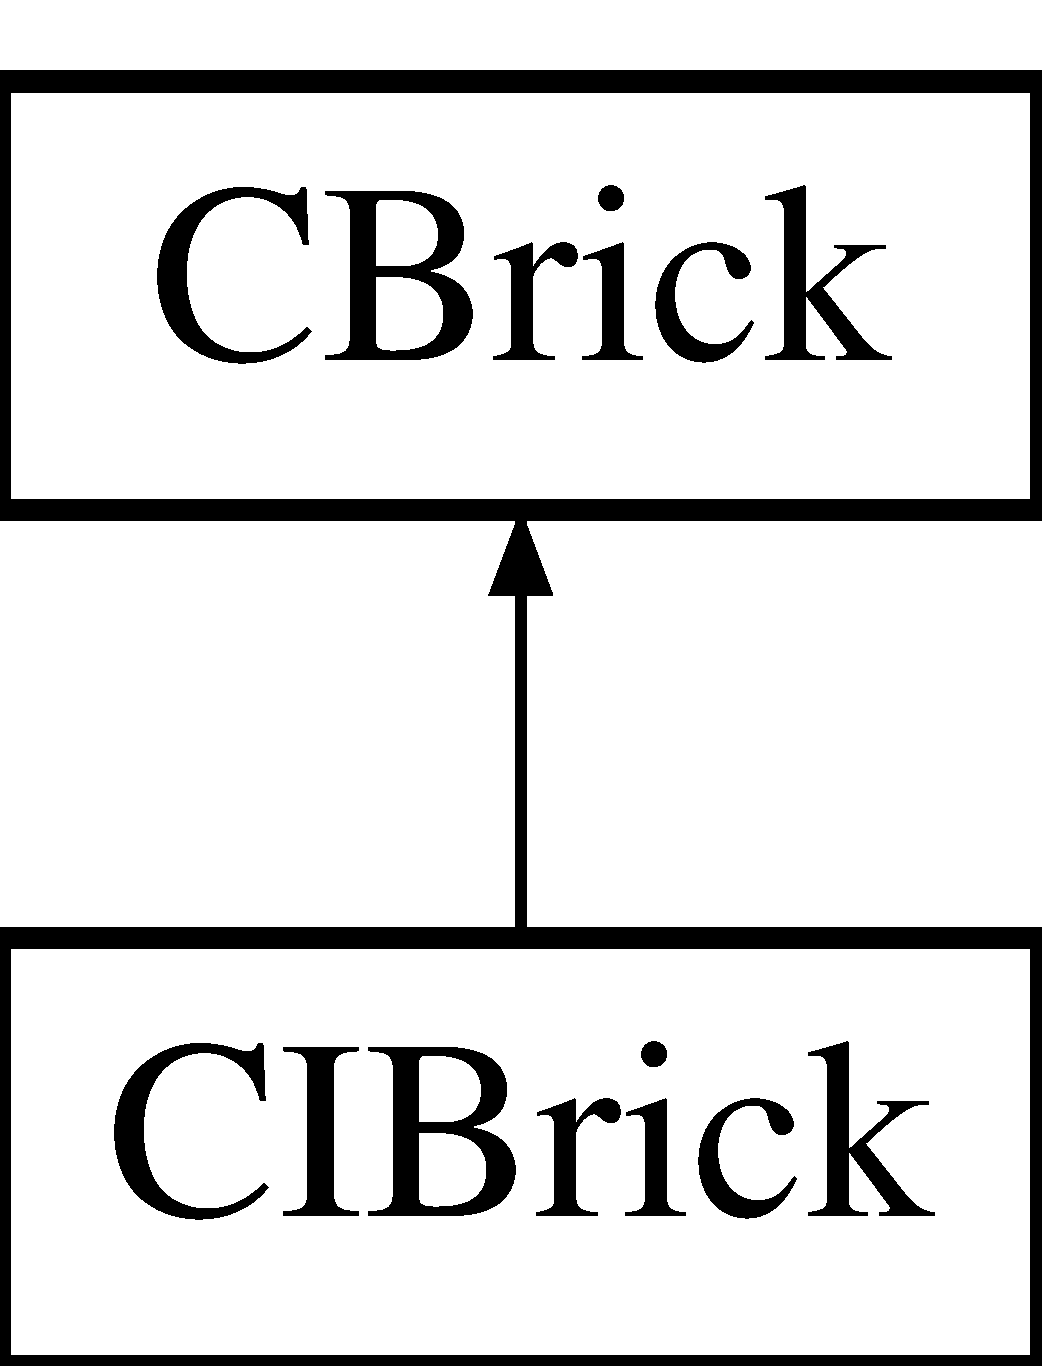
\includegraphics[height=2.000000cm]{classCIBrick}
\end{center}
\end{figure}
\subsection*{Public Member Functions}
\begin{DoxyCompactItemize}
\item 
\hypertarget{classCIBrick_a93ce36599370a04c1406f2474de28bff}{{\bfseries C\-I\-Brick} (const Direction direction=Direction\-::\-R)}\label{classCIBrick_a93ce36599370a04c1406f2474de28bff}

\item 
\hypertarget{classCIBrick_aa251c34a18be5c8433c35f1b5a99c669}{void {\bfseries Rotate} (const bool clock\-Wise=true)}\label{classCIBrick_aa251c34a18be5c8433c35f1b5a99c669}

\end{DoxyCompactItemize}
\subsection*{Additional Inherited Members}


The documentation for this class was generated from the following files\-:\begin{DoxyCompactItemize}
\item 
inc/Brick.\-h\item 
src/Brick.\-cpp\end{DoxyCompactItemize}

\hypertarget{classCLBrick}{\section{C\-L\-Brick Class Reference}
\label{classCLBrick}\index{C\-L\-Brick@{C\-L\-Brick}}
}
Inheritance diagram for C\-L\-Brick\-:\begin{figure}[H]
\begin{center}
\leavevmode
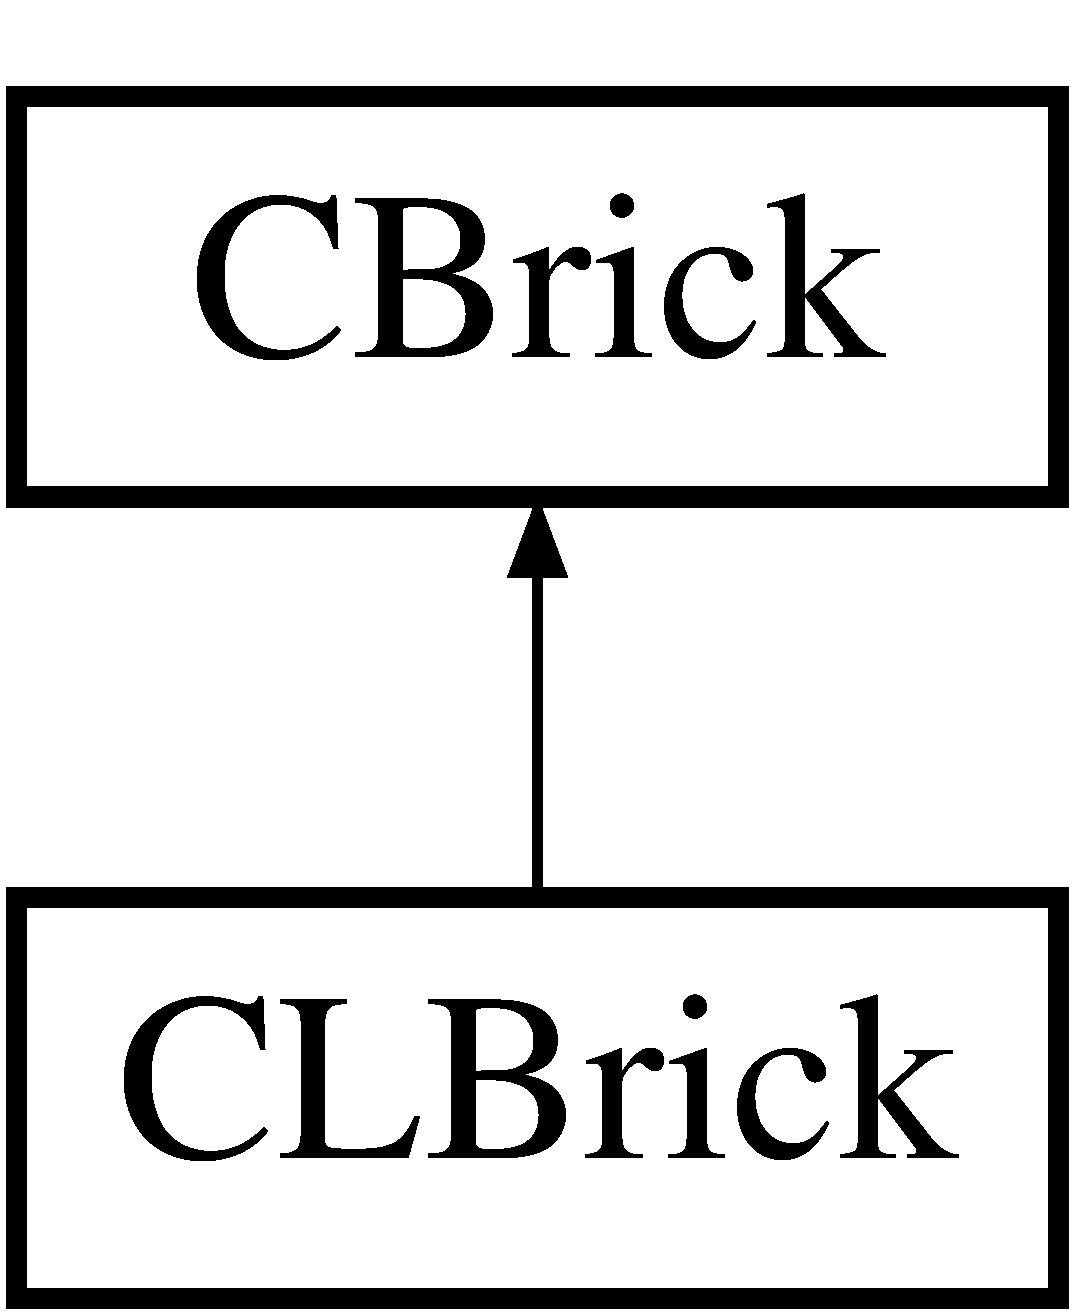
\includegraphics[height=2.000000cm]{classCLBrick}
\end{center}
\end{figure}
\subsection*{Public Member Functions}
\begin{DoxyCompactItemize}
\item 
\hypertarget{classCLBrick_a2e902d93bf6baa4bfbe2c99ceb85223e}{{\bfseries C\-L\-Brick} (const Direction direction=Direction\-::\-R)}\label{classCLBrick_a2e902d93bf6baa4bfbe2c99ceb85223e}

\item 
\hypertarget{classCLBrick_a78aaef2a95d9943faa1d0572ece28246}{void {\bfseries Rotate} (const bool clock\-Wise=true)}\label{classCLBrick_a78aaef2a95d9943faa1d0572ece28246}

\end{DoxyCompactItemize}
\subsection*{Additional Inherited Members}


The documentation for this class was generated from the following files\-:\begin{DoxyCompactItemize}
\item 
inc/Brick.\-h\item 
src/Brick.\-cpp\end{DoxyCompactItemize}

\hypertarget{classCMainGrid}{\section{C\-Main\-Grid Class Reference}
\label{classCMainGrid}\index{C\-Main\-Grid@{C\-Main\-Grid}}
}
\subsection*{Public Member Functions}
\begin{DoxyCompactItemize}
\item 
\hypertarget{classCMainGrid_a4cb57aa0aa8b37a466c5ad502dc04cb3}{{\bfseries C\-Main\-Grid} (C\-U\-Int rows\-Count=0, C\-U\-Int columns\-Count=0, C\-U\-Int initial\-X=0, C\-U\-Int initial\-Y=0)}\label{classCMainGrid_a4cb57aa0aa8b37a466c5ad502dc04cb3}

\item 
\hypertarget{classCMainGrid_a9051dc8159c06990b157238420e5c44a}{void {\bfseries Set\-Size} (C\-U\-Int rows\-Count, C\-U\-Int columns\-Count, C\-U\-Int initial\-X=0, C\-U\-Int initial\-Y=0)}\label{classCMainGrid_a9051dc8159c06990b157238420e5c44a}

\item 
\hypertarget{classCMainGrid_ad790fd79331041f0c82e3684bdd366d6}{void {\bfseries Set\-Background\-Picture} (const Path \&pic\-Location, C\-U\-Int width, C\-U\-Int height)}\label{classCMainGrid_ad790fd79331041f0c82e3684bdd366d6}

\item 
\hypertarget{classCMainGrid_a3d699794980df4ed55741802a5e6f99b}{void {\bfseries Set\-Slab\-Pic} (const Path \&pic\-Location, C\-U\-Int width, C\-U\-Int height)}\label{classCMainGrid_a3d699794980df4ed55741802a5e6f99b}

\item 
\hypertarget{classCMainGrid_a4a6c52b72b7bdffeb2c8501e17eef749}{void {\bfseries Add\-Brick} (const \hyperlink{classCBrick}{C\-Brick} \&brick)}\label{classCMainGrid_a4a6c52b72b7bdffeb2c8501e17eef749}

\item 
\hypertarget{classCMainGrid_a88ebd799daac44ebc6c6732d20423d15}{void {\bfseries Re\-Lease\-Brick} ()}\label{classCMainGrid_a88ebd799daac44ebc6c6732d20423d15}

\item 
\hypertarget{classCMainGrid_a75a4406abd98db7135ad063b13f50ff0}{C\-U\-Int {\bfseries Get\-Rows\-Count} () const }\label{classCMainGrid_a75a4406abd98db7135ad063b13f50ff0}

\item 
\hypertarget{classCMainGrid_af74282fc8abe5909ad1cf56fb77c97dd}{C\-U\-Int {\bfseries Get\-Columns\-Count} () const }\label{classCMainGrid_af74282fc8abe5909ad1cf56fb77c97dd}

\item 
\hypertarget{classCMainGrid_a603378af3ae46ed445d3f0e8f28311fd}{const String {\bfseries Slab\-Picture\-Loc} () const }\label{classCMainGrid_a603378af3ae46ed445d3f0e8f28311fd}

\item 
\hypertarget{classCMainGrid_afac1d7d3d43eb73832517bdf978b747c}{const String {\bfseries Empty\-Slab\-Picture\-Loc} () const }\label{classCMainGrid_afac1d7d3d43eb73832517bdf978b747c}

\item 
\hypertarget{classCMainGrid_a591e1a0371d94f7619e3dccee651ec5c}{C\-U\-Int {\bfseries Get\-Img\-Width} () const }\label{classCMainGrid_a591e1a0371d94f7619e3dccee651ec5c}

\item 
\hypertarget{classCMainGrid_a3da83bb820f0f41616fc5d966146ded4}{C\-U\-Int {\bfseries Get\-Img\-Height} () const }\label{classCMainGrid_a3da83bb820f0f41616fc5d966146ded4}

\item 
\hypertarget{classCMainGrid_ac474e39e99e6a247c8f1497128a9f27a}{C\-U\-Int {\bfseries Get\-Slab\-Row} (C\-U\-Int slab\-Index) const }\label{classCMainGrid_ac474e39e99e6a247c8f1497128a9f27a}

\item 
\hypertarget{classCMainGrid_ab3dd07039ffaa820097291c89aa167a3}{C\-U\-Int {\bfseries Get\-Slab\-Col} (C\-U\-Int slab\-Index) const }\label{classCMainGrid_ab3dd07039ffaa820097291c89aa167a3}

\item 
\hypertarget{classCMainGrid_aaa74bcd67f9466b0c83c09dbfd12d653}{const bool {\bfseries Part\-Of\-Slab} (C\-U\-Int slab\-Index) const }\label{classCMainGrid_aaa74bcd67f9466b0c83c09dbfd12d653}

\item 
\hypertarget{classCMainGrid_a298c29e33aa9792b61a883fd1201adc0}{const bool {\bfseries Empty} (C\-U\-Int row\-Index, C\-U\-Int col\-Index) const }\label{classCMainGrid_a298c29e33aa9792b61a883fd1201adc0}

\item 
\hypertarget{classCMainGrid_ad1d0e61bd6f8eadae1ea371d48379aac}{C\-U\-Int {\bfseries Slab\-Count} () const }\label{classCMainGrid_ad1d0e61bd6f8eadae1ea371d48379aac}

\item 
\hypertarget{classCMainGrid_a9885b198b38754f6a4f146da94b9583a}{const Coordinatest\-List {\bfseries Active\-Brick\-Coords} () const }\label{classCMainGrid_a9885b198b38754f6a4f146da94b9583a}

\item 
\hypertarget{classCMainGrid_a5989913dc3f69847b0487451228b3cf5}{const bool {\bfseries Slab\-Exist} (C\-U\-Int row\-Index, C\-U\-Int col\-Index) const }\label{classCMainGrid_a5989913dc3f69847b0487451228b3cf5}

\item 
\hypertarget{classCMainGrid_afedebf8cf7d6a059099d4570987027c8}{void {\bfseries Add\-Current\-Brick\-To\-Grid} ()}\label{classCMainGrid_afedebf8cf7d6a059099d4570987027c8}

\item 
\hypertarget{classCMainGrid_a4f7434247ade2231d257bc1c2860c96b}{const bool {\bfseries Part\-Of\-Current\-Brick} (C\-U\-Int row\-Index, C\-U\-Int col\-Index) const }\label{classCMainGrid_a4f7434247ade2231d257bc1c2860c96b}

\item 
\hypertarget{classCMainGrid_a16a1a3cde9ab2d8a4c2e3b367cf94034}{void {\bfseries Move\-Actual\-Brick} (const Direction direction)}\label{classCMainGrid_a16a1a3cde9ab2d8a4c2e3b367cf94034}

\item 
\hypertarget{classCMainGrid_af001df3b52aa8aa7091b59d15e2997ed}{const bool {\bfseries Check\-If\-Block\-Can\-Be\-Moved} (const Direction direction) const }\label{classCMainGrid_af001df3b52aa8aa7091b59d15e2997ed}

\item 
\hypertarget{classCMainGrid_ae77015d339f635b53921a74f2c8d42c4}{void {\bfseries Rotate\-Actual\-Brick} (const bool clock\-Wise=true)}\label{classCMainGrid_ae77015d339f635b53921a74f2c8d42c4}

\item 
\hypertarget{classCMainGrid_ab086114dfb0e40a4debd1205749347ab}{void {\bfseries Manage\-Full\-Line} ()}\label{classCMainGrid_ab086114dfb0e40a4debd1205749347ab}

\end{DoxyCompactItemize}


The documentation for this class was generated from the following files\-:\begin{DoxyCompactItemize}
\item 
inc/Main\-Grid.\-h\item 
src/Main\-Grid.\-cpp\end{DoxyCompactItemize}

\hypertarget{classCOBrick}{\section{C\-O\-Brick Class Reference}
\label{classCOBrick}\index{C\-O\-Brick@{C\-O\-Brick}}
}
Inheritance diagram for C\-O\-Brick\-:\begin{figure}[H]
\begin{center}
\leavevmode
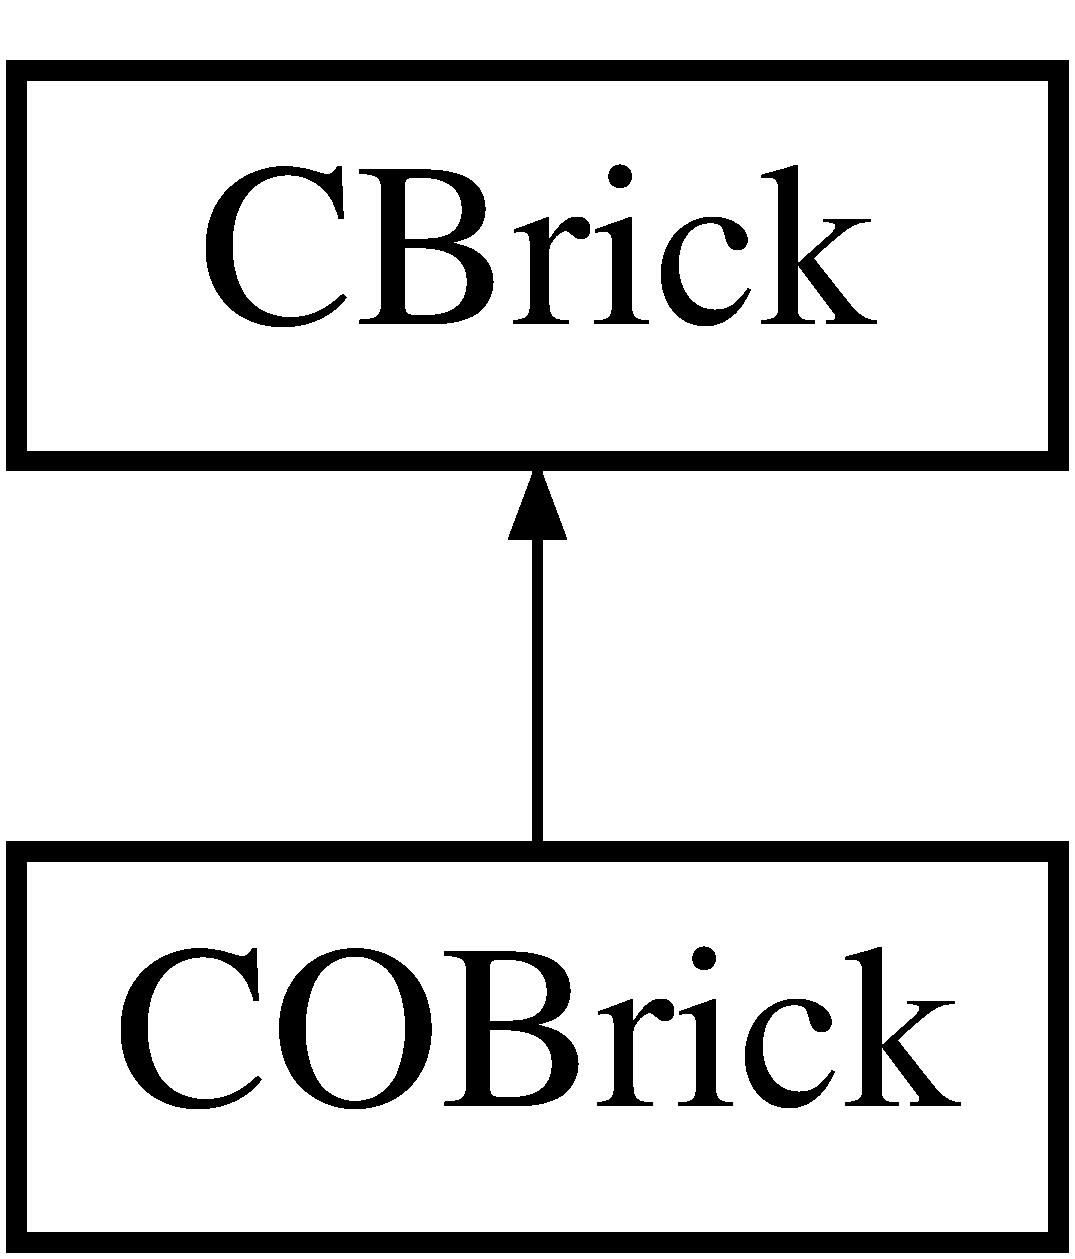
\includegraphics[height=2.000000cm]{classCOBrick}
\end{center}
\end{figure}
\subsection*{Public Member Functions}
\begin{DoxyCompactItemize}
\item 
\hypertarget{classCOBrick_ac6a97c2b05399ff04e8995c95eec5c0a}{{\bfseries C\-O\-Brick} (const Direction direction=Direction\-::\-R)}\label{classCOBrick_ac6a97c2b05399ff04e8995c95eec5c0a}

\item 
\hypertarget{classCOBrick_aa60947c3aa51e5fbb89965302153001e}{void {\bfseries Rotate} (const bool clock\-Wise=true)}\label{classCOBrick_aa60947c3aa51e5fbb89965302153001e}

\end{DoxyCompactItemize}
\subsection*{Additional Inherited Members}


The documentation for this class was generated from the following files\-:\begin{DoxyCompactItemize}
\item 
inc/Brick.\-h\item 
src/Brick.\-cpp\end{DoxyCompactItemize}

\hypertarget{classCOrientation}{\section{C\-Orientation Class Reference}
\label{classCOrientation}\index{C\-Orientation@{C\-Orientation}}
}
\subsection*{Public Types}
\begin{DoxyCompactItemize}
\item 
enum {\bfseries Direction} \{ {\bfseries L}, 
{\bfseries R}, 
{\bfseries U}, 
{\bfseries D}
 \}
\end{DoxyCompactItemize}
\subsection*{Public Member Functions}
\begin{DoxyCompactItemize}
\item 
\hypertarget{classCOrientation_a65116a9e6dc170a5d5690c3103fcf4a5}{{\bfseries C\-Orientation} (const Direction direction=R)}\label{classCOrientation_a65116a9e6dc170a5d5690c3103fcf4a5}

\item 
\hypertarget{classCOrientation_a505c222d112a1fc8c662955881fe5daa}{void {\bfseries Set} (const Direction direction)}\label{classCOrientation_a505c222d112a1fc8c662955881fe5daa}

\item 
\hypertarget{classCOrientation_a10e34c75395ce925cfb7ecf3e5c98adc}{const Direction {\bfseries Get} () const }\label{classCOrientation_a10e34c75395ce925cfb7ecf3e5c98adc}

\end{DoxyCompactItemize}


The documentation for this class was generated from the following files\-:\begin{DoxyCompactItemize}
\item 
inc/Orientation.\-h\item 
src/Orientation.\-cpp\end{DoxyCompactItemize}

\hypertarget{classCPicture}{\section{C\-Picture Class Reference}
\label{classCPicture}\index{C\-Picture@{C\-Picture}}
}
\subsection*{Public Member Functions}
\begin{DoxyCompactItemize}
\item 
\hypertarget{classCPicture_ab0aeabcb8789ee9f98cf86711cb7d709}{{\bfseries C\-Picture} (const Path \&location, const unsigned int width=10, const unsigned int height=10)}\label{classCPicture_ab0aeabcb8789ee9f98cf86711cb7d709}

\item 
\hypertarget{classCPicture_a00209611ef5fd84cd5acd867f9b6c89f}{void {\bfseries Draw} (const unsigned int x\-Post, const unsigned int y\-Pos)}\label{classCPicture_a00209611ef5fd84cd5acd867f9b6c89f}

\item 
\hypertarget{classCPicture_a3e98c0c303e309615fdc204792602f68}{\hyperlink{classCPicture}{C\-Picture} \& {\bfseries operator=} (const \hyperlink{classCPicture}{C\-Picture} \&picture)}\label{classCPicture_a3e98c0c303e309615fdc204792602f68}

\item 
\hypertarget{classCPicture_af7e2b2400001ecd701130a03ced37ce0}{void {\bfseries Set\-Picture\-Location} (const Path \&pic\-Location)}\label{classCPicture_af7e2b2400001ecd701130a03ced37ce0}

\item 
\hypertarget{classCPicture_a83f2b834109c9cbf33dfe790a5df2746}{void {\bfseries Set\-Picture\-Size} (const unsigned int width, const unsigned int height)}\label{classCPicture_a83f2b834109c9cbf33dfe790a5df2746}

\item 
\hypertarget{classCPicture_ab5934d9dbdfdfd0b03d9d137277d5115}{const String {\bfseries Get\-Img\-Loc} () const }\label{classCPicture_ab5934d9dbdfdfd0b03d9d137277d5115}

\item 
\hypertarget{classCPicture_a3c77bc3389f93d220a4af55f177b2fa8}{const unsigned int {\bfseries Get\-Img\-Width} () const }\label{classCPicture_a3c77bc3389f93d220a4af55f177b2fa8}

\item 
\hypertarget{classCPicture_aa5b4142c5ab12957e0df30a6c41dc5c5}{const unsigned int {\bfseries Get\-Img\-Height} () const }\label{classCPicture_aa5b4142c5ab12957e0df30a6c41dc5c5}

\end{DoxyCompactItemize}


The documentation for this class was generated from the following files\-:\begin{DoxyCompactItemize}
\item 
inc/Picture.\-h\item 
src/Picture.\-cpp\end{DoxyCompactItemize}

\hypertarget{classCPoint}{\section{C\-Point Class Reference}
\label{classCPoint}\index{C\-Point@{C\-Point}}
}
Inheritance diagram for C\-Point\-:\begin{figure}[H]
\begin{center}
\leavevmode
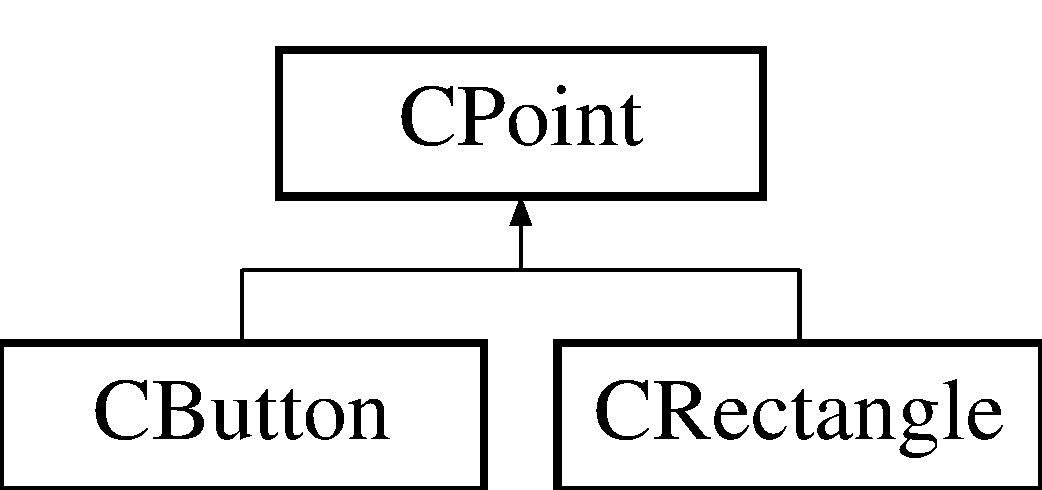
\includegraphics[height=2.000000cm]{classCPoint}
\end{center}
\end{figure}
\subsection*{Public Member Functions}
\begin{DoxyCompactItemize}
\item 
\hypertarget{classCPoint_ab11c86a3b00c3581d58a1c221256e112}{{\bfseries C\-Point} (const int x=0, const int y=0)}\label{classCPoint_ab11c86a3b00c3581d58a1c221256e112}

\item 
\hypertarget{classCPoint_a9307591d1d373653beeab949ff0f1ce6}{const int {\bfseries Get\-X} () const }\label{classCPoint_a9307591d1d373653beeab949ff0f1ce6}

\item 
\hypertarget{classCPoint_a6277e4683bbec2584925a24bcb2ad64f}{const int {\bfseries Get\-Y} () const }\label{classCPoint_a6277e4683bbec2584925a24bcb2ad64f}

\end{DoxyCompactItemize}


The documentation for this class was generated from the following files\-:\begin{DoxyCompactItemize}
\item 
inc/Point.\-h\item 
src/Point.\-cpp\end{DoxyCompactItemize}

\hypertarget{classCPosition}{\section{C\-Position Class Reference}
\label{classCPosition}\index{C\-Position@{C\-Position}}
}
\subsection*{Public Member Functions}
\begin{DoxyCompactItemize}
\item 
\hypertarget{classCPosition_a9e6eddbe9173d945fc75fc7493608663}{{\bfseries C\-Position} (C\-U\-Int x=0, C\-U\-Int y=0)}\label{classCPosition_a9e6eddbe9173d945fc75fc7493608663}

\item 
\hypertarget{classCPosition_a0d881df947c8609a2740fda0fd7d3c87}{{\bfseries C\-Position} (const \hyperlink{classCPosition}{C\-Position} \&position)}\label{classCPosition_a0d881df947c8609a2740fda0fd7d3c87}

\item 
\hypertarget{classCPosition_aadf42aa59912d16baef3639aa4706f35}{C\-U\-Int {\bfseries Get\-X} () const }\label{classCPosition_aadf42aa59912d16baef3639aa4706f35}

\item 
\hypertarget{classCPosition_acc5ed328ccc5d8f02e26313f9c902f00}{C\-U\-Int {\bfseries Get\-Y} () const }\label{classCPosition_acc5ed328ccc5d8f02e26313f9c902f00}

\item 
\hypertarget{classCPosition_a89cf175b15b096c7e4931b4e4adc0500}{\hyperlink{classCPosition}{C\-Position} \& {\bfseries operator=} (const \hyperlink{classCPosition}{C\-Position} \&position)}\label{classCPosition_a89cf175b15b096c7e4931b4e4adc0500}

\end{DoxyCompactItemize}


The documentation for this class was generated from the following files\-:\begin{DoxyCompactItemize}
\item 
inc/Position.\-h\item 
src/Position.\-cpp\end{DoxyCompactItemize}

\hypertarget{classCRectangle}{\section{C\-Rectangle Class Reference}
\label{classCRectangle}\index{C\-Rectangle@{C\-Rectangle}}
}
Inheritance diagram for C\-Rectangle\-:\begin{figure}[H]
\begin{center}
\leavevmode
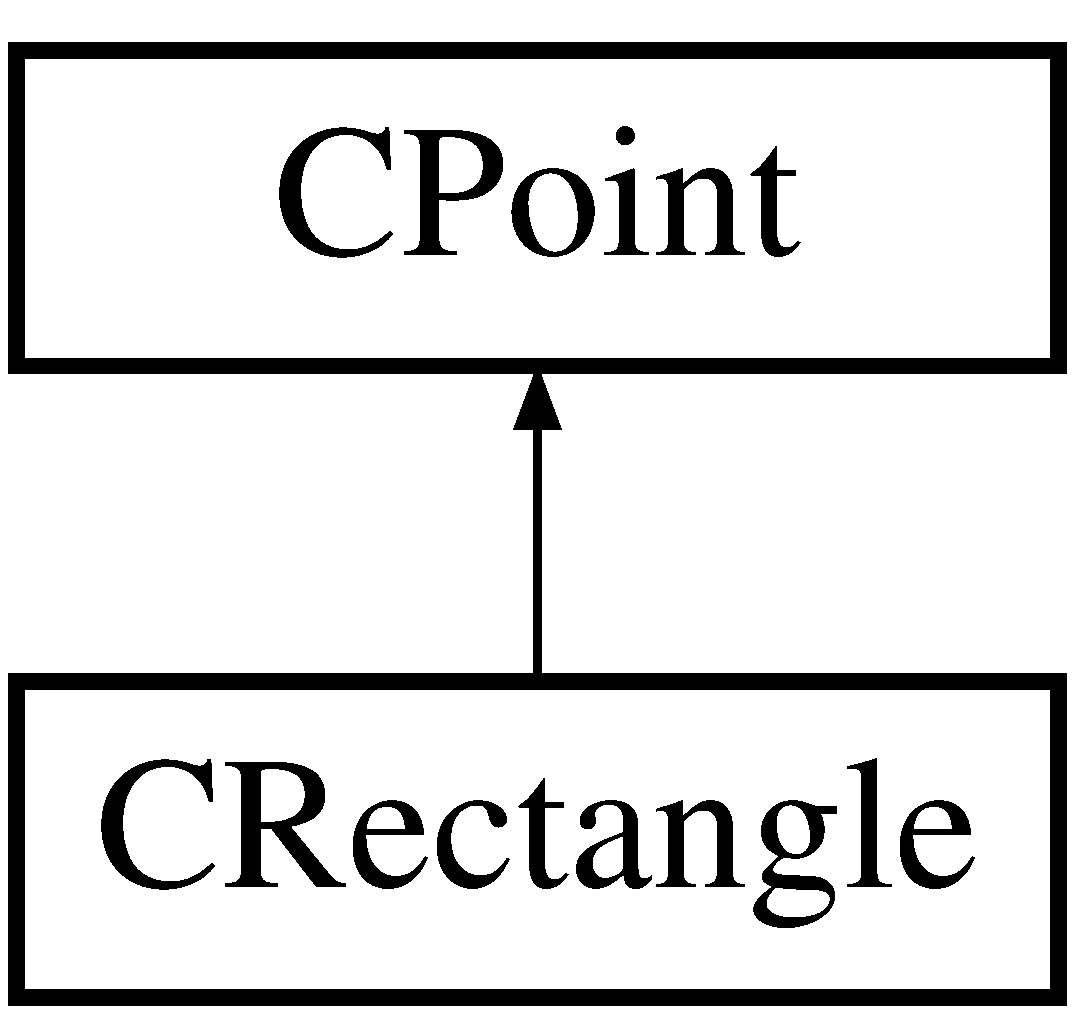
\includegraphics[height=2.000000cm]{classCRectangle}
\end{center}
\end{figure}
\subsection*{Public Member Functions}
\begin{DoxyCompactItemize}
\item 
\hypertarget{classCRectangle_aa0d285f137acc223be0bd1b0565d65ed}{{\bfseries C\-Rectangle} (C\-Intg x\-Pos=0, C\-Intg y\-Pos=0, C\-U\-Int width=0, C\-U\-Int height=0)}\label{classCRectangle_aa0d285f137acc223be0bd1b0565d65ed}

\item 
\hypertarget{classCRectangle_adc9c9c8d242dfcefb2016753e3b6f276}{C\-U\-Int {\bfseries Width} () const }\label{classCRectangle_adc9c9c8d242dfcefb2016753e3b6f276}

\item 
\hypertarget{classCRectangle_a7a94550650aa42f37595ab7120567c4a}{C\-U\-Int {\bfseries Height} () const }\label{classCRectangle_a7a94550650aa42f37595ab7120567c4a}

\end{DoxyCompactItemize}


The documentation for this class was generated from the following files\-:\begin{DoxyCompactItemize}
\item 
inc/Rectangle.\-h\item 
src/Rectangle.\-cpp\end{DoxyCompactItemize}

\hypertarget{classCSBrick}{\section{C\-S\-Brick Class Reference}
\label{classCSBrick}\index{C\-S\-Brick@{C\-S\-Brick}}
}
Inheritance diagram for C\-S\-Brick\-:\begin{figure}[H]
\begin{center}
\leavevmode
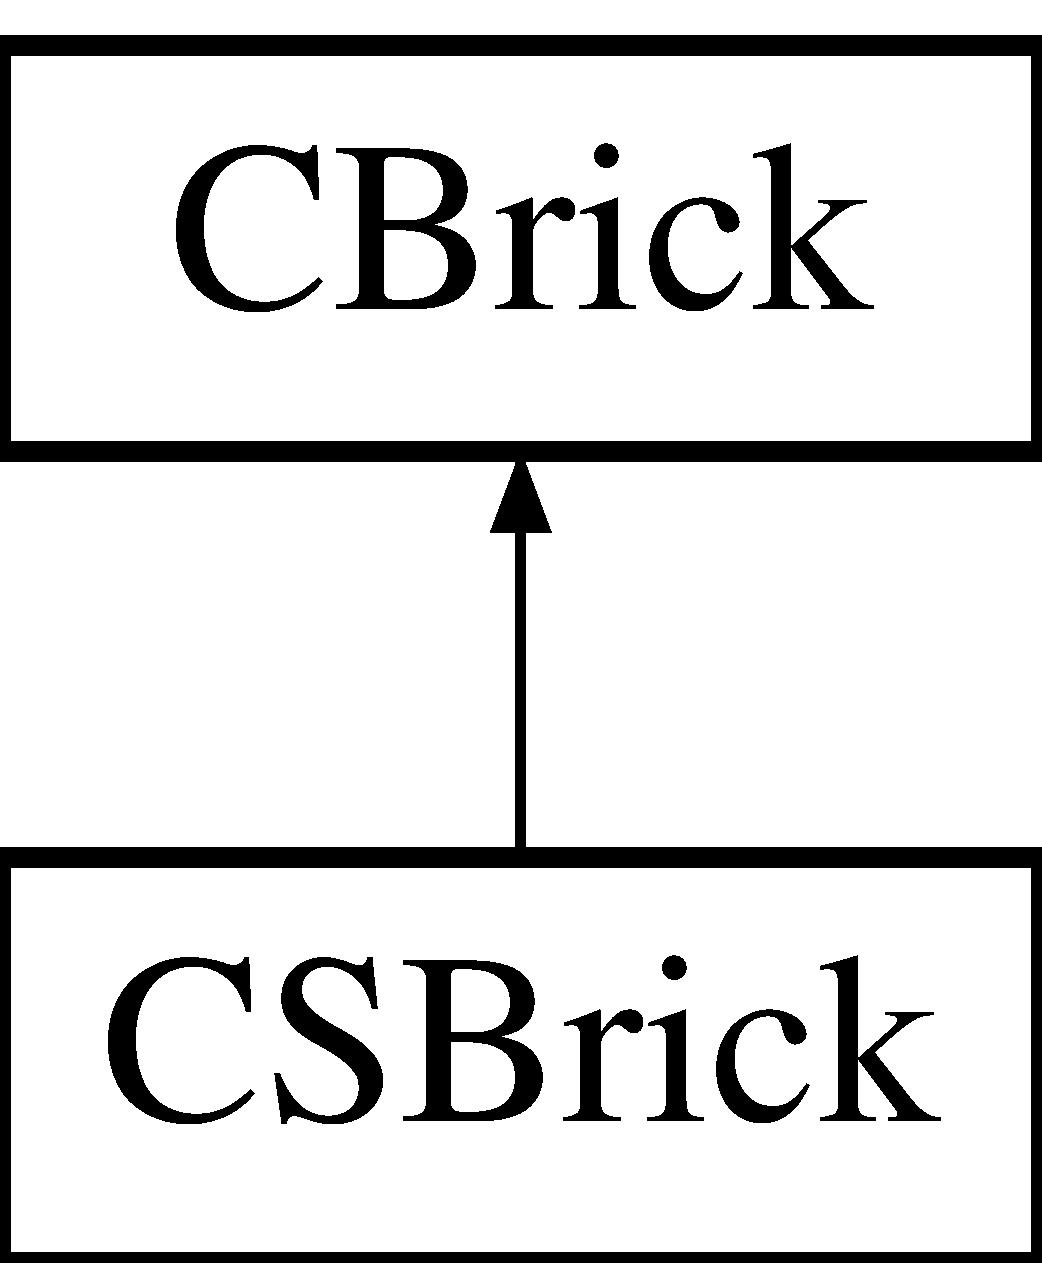
\includegraphics[height=2.000000cm]{classCSBrick}
\end{center}
\end{figure}
\subsection*{Public Member Functions}
\begin{DoxyCompactItemize}
\item 
\hypertarget{classCSBrick_a0abf72fc387548f5eee81c8cd10faedb}{{\bfseries C\-S\-Brick} (const Direction direction=Direction\-::\-R)}\label{classCSBrick_a0abf72fc387548f5eee81c8cd10faedb}

\item 
\hypertarget{classCSBrick_a0b3a43572caf4ee067b73aca65cc560f}{void {\bfseries Rotate} (const bool clock\-Wise=true)}\label{classCSBrick_a0b3a43572caf4ee067b73aca65cc560f}

\end{DoxyCompactItemize}
\subsection*{Additional Inherited Members}


The documentation for this class was generated from the following files\-:\begin{DoxyCompactItemize}
\item 
inc/Brick.\-h\item 
src/Brick.\-cpp\end{DoxyCompactItemize}

\hypertarget{classCSDLWrapper}{\section{C\-S\-D\-L\-Wrapper Class Reference}
\label{classCSDLWrapper}\index{C\-S\-D\-L\-Wrapper@{C\-S\-D\-L\-Wrapper}}
}
\subsection*{Public Member Functions}
\begin{DoxyCompactItemize}
\item 
\hypertarget{classCSDLWrapper_aad273110638082785f343eb090dc5d3c}{void {\bfseries Create\-Window} (C\-U\-Int width=0, C\-U\-Int height=0)}\label{classCSDLWrapper_aad273110638082785f343eb090dc5d3c}

\item 
\hypertarget{classCSDLWrapper_a9579a55f0a9a7ea676935bdbd8cf46ea}{void {\bfseries Add\-Image} (const String \&path)}\label{classCSDLWrapper_a9579a55f0a9a7ea676935bdbd8cf46ea}

\item 
\hypertarget{classCSDLWrapper_ae58baf0891ce060ce9505ab25a46b7b7}{void {\bfseries Apply\-Image} (C\-U\-Int img\-Index, C\-U\-Int x, C\-U\-Int y)}\label{classCSDLWrapper_ae58baf0891ce060ce9505ab25a46b7b7}

\item 
\hypertarget{classCSDLWrapper_aa227a005cc9ff099b3cb3b698d7bb925}{void {\bfseries Display} (const \hyperlink{classCMainGrid}{C\-Main\-Grid} \&grid)}\label{classCSDLWrapper_aa227a005cc9ff099b3cb3b698d7bb925}

\item 
\hypertarget{classCSDLWrapper_aff7ea8946d30fe7e8c00966155f536a6}{void {\bfseries Display} (const \hyperlink{classCButton}{C\-Button} \&button)}\label{classCSDLWrapper_aff7ea8946d30fe7e8c00966155f536a6}

\item 
\hypertarget{classCSDLWrapper_a22206e6af4087a884970ba1800feb224}{void {\bfseries Actualize} ()}\label{classCSDLWrapper_a22206e6af4087a884970ba1800feb224}

\item 
\hypertarget{classCSDLWrapper_a44e500f2b108ad52dd5e0585ac3483c2}{void {\bfseries Main\-Loop} ()}\label{classCSDLWrapper_a44e500f2b108ad52dd5e0585ac3483c2}

\end{DoxyCompactItemize}
\subsection*{Static Public Member Functions}
\begin{DoxyCompactItemize}
\item 
\hypertarget{classCSDLWrapper_aafff4b431f939fe21143122b5ade38c5}{static \hyperlink{classCSDLWrapper}{C\-S\-D\-L\-Wrapper} $\ast$ {\bfseries Instance} ()}\label{classCSDLWrapper_aafff4b431f939fe21143122b5ade38c5}

\item 
\hypertarget{classCSDLWrapper_a4a40a3eb7da79638f98a95e7b5bd20d0}{static void {\bfseries Destroy} ()}\label{classCSDLWrapper_a4a40a3eb7da79638f98a95e7b5bd20d0}

\end{DoxyCompactItemize}


The documentation for this class was generated from the following files\-:\begin{DoxyCompactItemize}
\item 
inc/S\-D\-L\-Wrapper.\-h\item 
src/S\-D\-L\-Wrapper.\-cpp\end{DoxyCompactItemize}

\hypertarget{classCSlab}{\section{C\-Slab Class Reference}
\label{classCSlab}\index{C\-Slab@{C\-Slab}}
}
\subsection*{Public Member Functions}
\begin{DoxyCompactItemize}
\item 
\hypertarget{classCSlab_a78323aeb9b867b56c5ec46174f5379b6}{{\bfseries C\-Slab} (const \hyperlink{classCSlab}{C\-Slab} \&slab)}\label{classCSlab_a78323aeb9b867b56c5ec46174f5379b6}

\item 
\hypertarget{classCSlab_abd74b162e714d6ec9f6b049ff4e32aa6}{{\bfseries C\-Slab} (C\-U\-Int row=0, C\-U\-Int col=0, const bool part\-Of\-Slab=false, const bool empty=true)}\label{classCSlab_abd74b162e714d6ec9f6b049ff4e32aa6}

\item 
\hypertarget{classCSlab_a20e487ca68e69810cd34a2775d03f23e}{\hyperlink{classCSlab}{C\-Slab} \& {\bfseries operator=} (const \hyperlink{classCSlab}{C\-Slab} \&slab)}\label{classCSlab_a20e487ca68e69810cd34a2775d03f23e}

\item 
\hypertarget{classCSlab_ac00a40725a72a34c05b01d6a9a19e8a6}{C\-U\-Int {\bfseries Row} () const }\label{classCSlab_ac00a40725a72a34c05b01d6a9a19e8a6}

\item 
\hypertarget{classCSlab_a0681fc1f984691e6d0eb43515c179cfe}{C\-U\-Int {\bfseries Col} () const }\label{classCSlab_a0681fc1f984691e6d0eb43515c179cfe}

\item 
\hypertarget{classCSlab_afb073bcd8717a05be1b308001b967f6c}{void {\bfseries Row} (C\-U\-Int row)}\label{classCSlab_afb073bcd8717a05be1b308001b967f6c}

\item 
\hypertarget{classCSlab_a5ae44b90c30e868bb63e5fc90bcbbe26}{void {\bfseries Col} (C\-U\-Int col)}\label{classCSlab_a5ae44b90c30e868bb63e5fc90bcbbe26}

\item 
\hypertarget{classCSlab_a14b5fa52b52ad1c32228b815bd7779b3}{void {\bfseries Set\-Position} (C\-U\-Int row, C\-U\-Int col)}\label{classCSlab_a14b5fa52b52ad1c32228b815bd7779b3}

\item 
\hypertarget{classCSlab_a776b5e80c09215694dfd3c0fb6cf13c7}{const bool {\bfseries Part\-Of\-Slab} () const }\label{classCSlab_a776b5e80c09215694dfd3c0fb6cf13c7}

\item 
\hypertarget{classCSlab_a9e84286ba37ec4c4c6707303ce4c7dbc}{void {\bfseries Part\-Of\-Slab} (const bool part\-Of\-Slab)}\label{classCSlab_a9e84286ba37ec4c4c6707303ce4c7dbc}

\item 
\hypertarget{classCSlab_afe56c35268d3c8edd8bad05fd44662fb}{const bool {\bfseries Empty} () const }\label{classCSlab_afe56c35268d3c8edd8bad05fd44662fb}

\item 
\hypertarget{classCSlab_a34b2bd7c751c80f9e79fd99a289686d5}{void {\bfseries Empty} (const bool empty)}\label{classCSlab_a34b2bd7c751c80f9e79fd99a289686d5}

\end{DoxyCompactItemize}


The documentation for this class was generated from the following files\-:\begin{DoxyCompactItemize}
\item 
inc/Slab.\-h\item 
src/Slab.\-cpp\end{DoxyCompactItemize}

\hypertarget{classCTableCoor}{\section{C\-Table\-Coor Class Reference}
\label{classCTableCoor}\index{C\-Table\-Coor@{C\-Table\-Coor}}
}
\subsection*{Public Member Functions}
\begin{DoxyCompactItemize}
\item 
\hypertarget{classCTableCoor_a563cdff97f0d7845be0bac884c2ee4b8}{{\bfseries C\-Table\-Coor} (C\-U\-Int row, C\-U\-Int column)}\label{classCTableCoor_a563cdff97f0d7845be0bac884c2ee4b8}

\item 
\hypertarget{classCTableCoor_a9766e415c31d1fc93686680b95387278}{C\-U\-Int {\bfseries Row} () const }\label{classCTableCoor_a9766e415c31d1fc93686680b95387278}

\item 
\hypertarget{classCTableCoor_a9efb127e100fe0c2c60879fe24cc0e96}{C\-U\-Int {\bfseries Col} () const }\label{classCTableCoor_a9efb127e100fe0c2c60879fe24cc0e96}

\item 
\hypertarget{classCTableCoor_a1c0578a6b9028bfa3667c4157f8b6cb0}{void {\bfseries Row} (C\-U\-Int row)}\label{classCTableCoor_a1c0578a6b9028bfa3667c4157f8b6cb0}

\item 
\hypertarget{classCTableCoor_a06a9f17cdd0f93d878c81d411cc9ec49}{void {\bfseries Col} (C\-U\-Int col)}\label{classCTableCoor_a06a9f17cdd0f93d878c81d411cc9ec49}

\item 
\hypertarget{classCTableCoor_af61a668edc8d8ddffca9ec5ad1ef508a}{void {\bfseries Change\-Position} (C\-U\-Int row, C\-U\-Int col)}\label{classCTableCoor_af61a668edc8d8ddffca9ec5ad1ef508a}

\item 
\hypertarget{classCTableCoor_ab55b738e5cc37d397de79d353d7a35f9}{\hyperlink{classCTableCoor}{C\-Table\-Coor} \& {\bfseries operator=} (const \hyperlink{classCTableCoor}{C\-Table\-Coor} \&coor)}\label{classCTableCoor_ab55b738e5cc37d397de79d353d7a35f9}

\end{DoxyCompactItemize}


The documentation for this class was generated from the following files\-:\begin{DoxyCompactItemize}
\item 
inc/Table\-Coordinates.\-h\item 
src/Table\-Coordinates.\-cpp\end{DoxyCompactItemize}

\hypertarget{classCTBrick}{\section{C\-T\-Brick Class Reference}
\label{classCTBrick}\index{C\-T\-Brick@{C\-T\-Brick}}
}
Inheritance diagram for C\-T\-Brick\-:\begin{figure}[H]
\begin{center}
\leavevmode
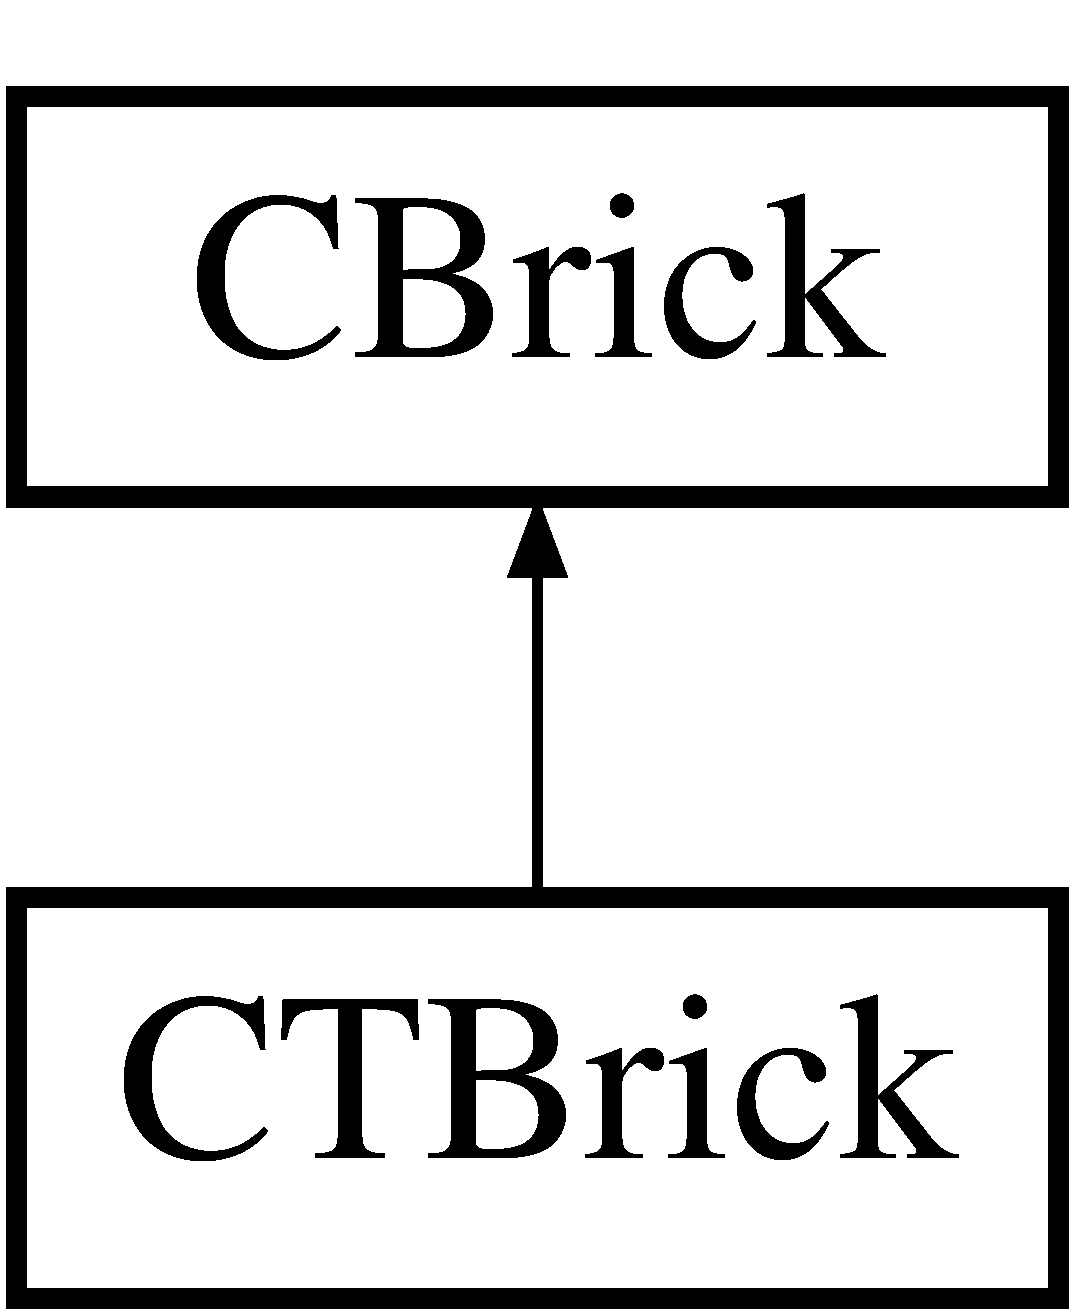
\includegraphics[height=2.000000cm]{classCTBrick}
\end{center}
\end{figure}
\subsection*{Public Member Functions}
\begin{DoxyCompactItemize}
\item 
\hypertarget{classCTBrick_ac33acf0e990eb86498a35b9c055e2395}{{\bfseries C\-T\-Brick} (const Direction direction=Direction\-::\-R)}\label{classCTBrick_ac33acf0e990eb86498a35b9c055e2395}

\item 
\hypertarget{classCTBrick_ae13cd4cbb5b8305bd5c7b5e6a34a3ad9}{void {\bfseries Rotate} (const bool clock\-Wise=true)}\label{classCTBrick_ae13cd4cbb5b8305bd5c7b5e6a34a3ad9}

\end{DoxyCompactItemize}
\subsection*{Additional Inherited Members}


The documentation for this class was generated from the following files\-:\begin{DoxyCompactItemize}
\item 
inc/Brick.\-h\item 
src/Brick.\-cpp\end{DoxyCompactItemize}

\hypertarget{classCTimeMod}{\section{C\-Time\-Mod Class Reference}
\label{classCTimeMod}\index{C\-Time\-Mod@{C\-Time\-Mod}}
}
\subsection*{Static Public Member Functions}
\begin{DoxyCompactItemize}
\item 
\hypertarget{classCTimeMod_a000f599005c02e227d44b7aab40ddd34}{static void {\bfseries Sleep\-Seconds} (C\-U\-Int seconds)}\label{classCTimeMod_a000f599005c02e227d44b7aab40ddd34}

\item 
\hypertarget{classCTimeMod_ac56c75a7f0db65d77bea3aef776be346}{static void {\bfseries Sleep\-Mili\-Seconds} (C\-U\-Int m\-Seconds)}\label{classCTimeMod_ac56c75a7f0db65d77bea3aef776be346}

\end{DoxyCompactItemize}


The documentation for this class was generated from the following files\-:\begin{DoxyCompactItemize}
\item 
inc/M\-Time.\-h\item 
src/M\-Time.\-cpp\end{DoxyCompactItemize}

%--- End generated contents ---

% Index
\newpage
\phantomsection
\addcontentsline{toc}{chapter}{Index}
\printindex

\end{document}
